%% bare_jrnl.tex
%% V1.4b
%% 2015/08/26
%% by Michael Shell
%% see http://www.michaelshell.org/
%% for current contact information.
%%
%% This is a skeleton file demonstrating the use of IEEEtran.cls
%% (requires IEEEtran.cls version 1.8b or later) with an IEEE
%% journal paper.
%%
%% Support sites:
%% http://www.michaelshell.org/tex/ieeetran/
%% http://www.ctan.org/pkg/ieeetran
%% and
%% http://www.ieee.org/

%%*************************************************************************
%% Legal Notice:
%% This code is offered as-is without any warranty either expressed or
%% implied; without even the implied warranty of MERCHANTABILITY or
%% FITNESS FOR A PARTICULAR PURPOSE! 
%% User assumes all risk.
%% In no event shall the IEEE or any contributor to this code be liable for
%% any damages or losses, including, but not limited to, incidental,
%% consequential, or any other damages, resulting from the use or misuse
%% of any information contained here.
%%
%% All comments are the opinions of their respective authors and are not
%% necessarily endorsed by the IEEE.
%%
%% This work is distributed under the LaTeX Project Public License (LPPL)
%% ( http://www.latex-project.org/ ) version 1.3, and may be freely used,
%% distributed and modified. A copy of the LPPL, version 1.3, is included
%% in the base LaTeX documentation of all distributions of LaTeX released
%% 2003/12/01 or later.
%% Retain all contribution notices and credits.
%% ** Modified files should be clearly indicated as such, including  **
%% ** renaming them and changing author support contact information. **
%%*************************************************************************


% *** Authors should verify (and, if needed, correct) their LaTeX system  ***
% *** with the testflow diagnostic prior to trusting their LaTeX platform ***
% *** with production work. The IEEE's font choices and paper sizes can   ***
% *** trigger bugs that do not appear when using other class files.       ***                          ***
% The testflow support page is at:
% http://www.michaelshell.org/tex/testflow/



\documentclass[journal]{IEEEtran}
%
% If IEEEtran.cls has not been installed into the LaTeX system files,
% manually specify the path to it like:
% \documentclass[journal]{../sty/IEEEtran}





% Some very useful LaTeX packages include:
% (uncomment the ones you want to load)


% *** MISC UTILITY PACKAGES ***
%
%\usepackage{ifpdf}
% Heiko Oberdiek's ifpdf.sty is very useful if you need conditional
% compilation based on whether the output is pdf or dvi.
% usage:
% \ifpdf
%   % pdf code
% \else
%   % dvi code
% \fi
% The latest version of ifpdf.sty can be obtained from:
% http://www.ctan.org/pkg/ifpdf
% Also, note that IEEEtran.cls V1.7 and later provides a builtin
% \ifCLASSINFOpdf conditional that works the same way.
% When switching from latex to pdflatex and vice-versa, the compiler may
% have to be run twice to clear warning/error messages.






% *** CITATION PACKAGES ***
%
%\usepackage{cite}
% cite.sty was written by Donald Arseneau
% V1.6 and later of IEEEtran pre-defines the format of the cite.sty package
% \cite{} output to follow that of the IEEE. Loading the cite package will
% result in citation numbers being automatically sorted and properly
% "compressed/ranged". e.g., [1], [9], [2], [7], [5], [6] without using
% cite.sty will become [1], [2], [5]--[7], [9] using cite.sty. cite.sty's
% \cite will automatically add leading space, if needed. Use cite.sty's
% noadjust option (cite.sty V3.8 and later) if you want to turn this off
% such as if a citation ever needs to be enclosed in parenthesis.
% cite.sty is already installed on most LaTeX systems. Be sure and use
% version 5.0 (2009-03-20) and later if using hyperref.sty.
% The latest version can be obtained at:
% http://www.ctan.org/pkg/cite
% The documentation is contained in the cite.sty file itself.






% *** GRAPHICS RELATED PACKAGES ***
%
\ifCLASSINFOpdf
  % \usepackage[pdftex]{graphicx}
  % declare the path(s) where your graphic files are
  % \graphicspath{{../pdf/}{../jpeg/}}
  % and their extensions so you won't have to specify these with
  % every instance of \includegraphics
  % \DeclareGraphicsExtensions{.pdf,.jpeg,.png}
\else
  % or other class option (dvipsone, dvipdf, if not using dvips). graphicx
  % will default to the driver specified in the system graphics.cfg if no
  % driver is specified.
  % \usepackage[dvips]{graphicx}
  % declare the path(s) where your graphic files are
  % \graphicspath{{../eps/}}
  % and their extensions so you won't have to specify these with
  % every instance of \includegraphics
  % \DeclareGraphicsExtensions{.eps}
\fi
% graphicx was written by David Carlisle and Sebastian Rahtz. It is
% required if you want graphics, photos, etc. graphicx.sty is already
% installed on most LaTeX systems. The latest version and documentation
% can be obtained at: 
% http://www.ctan.org/pkg/graphicx
% Another good source of documentation is "Using Imported Graphics in
% LaTeX2e" by Keith Reckdahl which can be found at:
% http://www.ctan.org/pkg/epslatex
%
% latex, and pdflatex in dvi mode, support graphics in encapsulated
% postscript (.eps) format. pdflatex in pdf mode supports graphics
% in .pdf, .jpeg, .png and .mps (metapost) formats. Users should ensure
% that all non-photo figures use a vector format (.eps, .pdf, .mps) and
% not a bitmapped formats (.jpeg, .png). The IEEE frowns on bitmapped formats
% which can result in "jaggedy"/blurry rendering of lines and letters as
% well as large increases in file sizes.
%
% You can find documentation about the pdfTeX application at:
% http://www.tug.org/applications/pdftex





% *** MATH PACKAGES ***
%
%\usepackage{amsmath}
% A popular package from the American Mathematical Society that provides
% many useful and powerful commands for dealing with mathematics.
%
% Note that the amsmath package sets \interdisplaylinepenalty to 10000
% thus preventing page breaks from occurring within multiline equations. Use:
%\interdisplaylinepenalty=2500
% after loading amsmath to restore such page breaks as IEEEtran.cls normally
% does. amsmath.sty is already installed on most LaTeX systems. The latest
% version and documentation can be obtained at:
% http://www.ctan.org/pkg/amsmath





% *** SPECIALIZED LIST PACKAGES ***
%
%\usepackage{algorithmic}
% algorithmic.sty was written by Peter Williams and Rogerio Brito.
% This package provides an algorithmic environment fo describing algorithms.
% You can use the algorithmic environment in-text or within a figure
% environment to provide for a floating algorithm. Do NOT use the algorithm
% floating environment provided by algorithm.sty (by the same authors) or
% algorithm2e.sty (by Christophe Fiorio) as the IEEE does not use dedicated
% algorithm float types and packages that provide these will not provide
% correct IEEE style captions. The latest version and documentation of
% algorithmic.sty can be obtained at:
% http://www.ctan.org/pkg/algorithms
% Also of interest may be the (relatively newer and more customizable)
% algorithmicx.sty package by Szasz Janos:
% http://www.ctan.org/pkg/algorithmicx




% *** ALIGNMENT PACKAGES ***
%
%\usepackage{array}
% Frank Mittelbach's and David Carlisle's array.sty patches and improves
% the standard LaTeX2e array and tabular environments to provide better
% appearance and additional user controls. As the default LaTeX2e table
% generation code is lacking to the point of almost being broken with
% respect to the quality of the end results, all users are strongly
% advised to use an enhanced (at the very least that provided by array.sty)
% set of table tools. array.sty is already installed on most systems. The
% latest version and documentation can be obtained at:
% http://www.ctan.org/pkg/array


% IEEEtran contains the IEEEeqnarray family of commands that can be used to
% generate multiline equations as well as matrices, tables, etc., of high
% quality.




% *** SUBFIGURE PACKAGES ***
%\ifCLASSOPTIONcompsoc
%  \usepackage[caption=false,font=normalsize,labelfont=sf,textfont=sf]{subfig}
%\else
%  \usepackage[caption=false,font=footnotesize]{subfig}
%\fi
% subfig.sty, written by Steven Douglas Cochran, is the modern replacement
% for subfigure.sty, the latter of which is no longer maintained and is
% incompatible with some LaTeX packages including fixltx2e. However,
% subfig.sty requires and automatically loads Axel Sommerfeldt's caption.sty
% which will override IEEEtran.cls' handling of captions and this will result
% in non-IEEE style figure/table captions. To prevent this problem, be sure
% and invoke subfig.sty's "caption=false" package option (available since
% subfig.sty version 1.3, 2005/06/28) as this is will preserve IEEEtran.cls
% handling of captions.
% Note that the Computer Society format requires a larger sans serif font
% than the serif footnote size font used in traditional IEEE formatting
% and thus the need to invoke different subfig.sty package options depending
% on whether compsoc mode has been enabled.
%
% The latest version and documentation of subfig.sty can be obtained at:
% http://www.ctan.org/pkg/subfig




% *** FLOAT PACKAGES ***
%
%\usepackage{fixltx2e}
% fixltx2e, the successor to the earlier fix2col.sty, was written by
% Frank Mittelbach and David Carlisle. This package corrects a few problems
% in the LaTeX2e kernel, the most notable of which is that in current
% LaTeX2e releases, the ordering of single and double column floats is not
% guaranteed to be preserved. Thus, an unpatched LaTeX2e can allow a
% single column figure to be placed prior to an earlier double column
% figure.
% Be aware that LaTeX2e kernels dated 2015 and later have fixltx2e.sty's
% corrections already built into the system in which case a warning will
% be issued if an attempt is made to load fixltx2e.sty as it is no longer
% needed.
% The latest version and documentation can be found at:
% http://www.ctan.org/pkg/fixltx2e


%\usepackage{stfloats}
% stfloats.sty was written by Sigitas Tolusis. This package gives LaTeX2e
% the ability to do double column floats at the bottom of the page as well
% as the top. (e.g., "\begin{figure*}[!b]" is not normally possible in
% LaTeX2e). It also provides a command:
%\fnbelowfloat
% to enable the placement of footnotes below bottom floats (the standard
% LaTeX2e kernel puts them above bottom floats). This is an invasive package
% which rewrites many portions of the LaTeX2e float routines. It may not work
% with other packages that modify the LaTeX2e float routines. The latest
% version and documentation can be obtained at:
% http://www.ctan.org/pkg/stfloats
% Do not use the stfloats baselinefloat ability as the IEEE does not allow
% \baselineskip to stretch. Authors submitting work to the IEEE should note
% that the IEEE rarely uses double column equations and that authors should try
% to avoid such use. Do not be tempted to use the cuted.sty or midfloat.sty
% packages (also by Sigitas Tolusis) as the IEEE does not format its papers in
% such ways.
% Do not attempt to use stfloats with fixltx2e as they are incompatible.
% Instead, use Morten Hogholm'a dblfloatfix which combines the features
% of both fixltx2e and stfloats:
%
% \usepackage{dblfloatfix}
% The latest version can be found at:
% http://www.ctan.org/pkg/dblfloatfix




%\ifCLASSOPTIONcaptionsoff
%  \usepackage[nomarkers]{endfloat}
% \let\MYoriglatexcaption\caption
% \renewcommand{\caption}[2][\relax]{\MYoriglatexcaption[#2]{#2}}
%\fi
% endfloat.sty was written by James Darrell McCauley, Jeff Goldberg and 
% Axel Sommerfeldt. This package may be useful when used in conjunction with 
% IEEEtran.cls'  captionsoff option. Some IEEE journals/societies require that
% submissions have lists of figures/tables at the end of the paper and that
% figures/tables without any captions are placed on a page by themselves at
% the end of the document. If needed, the draftcls IEEEtran class option or
% \CLASSINPUTbaselinestretch interface can be used to increase the line
% spacing as well. Be sure and use the nomarkers option of endfloat to
% prevent endfloat from "marking" where the figures would have been placed
% in the text. The two hack lines of code above are a slight modification of
% that suggested by in the endfloat docs (section 8.4.1) to ensure that
% the full captions always appear in the list of figures/tables - even if
% the user used the short optional argument of \caption[]{}.
% IEEE papers do not typically make use of \caption[]'s optional argument,
% so this should not be an issue. A similar trick can be used to disable
% captions of packages such as subfig.sty that lack options to turn off
% the subcaptions:
% For subfig.sty:
% \let\MYorigsubfloat\subfloat
% \renewcommand{\subfloat}[2][\relax]{\MYorigsubfloat[]{#2}}
% However, the above trick will not work if both optional arguments of
% the \subfloat command are used. Furthermore, there needs to be a
% description of each subfigure *somewhere* and endfloat does not add
% subfigure captions to its list of figures. Thus, the best approach is to
% avoid the use of subfigure captions (many IEEE journals avoid them anyway)
% and instead reference/explain all the subfigures within the main caption.
% The latest version of endfloat.sty and its documentation can obtained at:
% http://www.ctan.org/pkg/endfloat
%
% The IEEEtran \ifCLASSOPTIONcaptionsoff conditional can also be used
% later in the document, say, to conditionally put the References on a 
% page by themselves.




% *** PDF, URL AND HYPERLINK PACKAGES ***
%
%\usepackage{url}
% url.sty was written by Donald Arseneau. It provides better support for
% handling and breaking URLs. url.sty is already installed on most LaTeX
% systems. The latest version and documentation can be obtained at:
% http://www.ctan.org/pkg/url
% Basically, \url{my_url_here}.




% *** Do not adjust lengths that control margins, column widths, etc. ***
% *** Do not use packages that alter fonts (such as pslatex).         ***
% There should be no need to do such things with IEEEtran.cls V1.6 and later.
% (Unless specifically asked to do so by the journal or conference you plan
% to submit to, of course. )
\usepackage{amsmath,amsthm}
\usepackage{graphicx}
\usepackage{amsfonts}
\usepackage{algorithm}
\usepackage{algpseudocode}%
%\usepackage[title]{appendix}%
\usepackage{listings}%
\usepackage{xcolor}%
\usepackage{textcomp}%
\usepackage{manyfoot}%
\usepackage{booktabs}%
\usepackage{url}
\usepackage{cite}
%\usepackage{algpseudocode}
%\usepackage{booktabs}
\usepackage{tikz}
%\usepackage{natbib}
%\usetikzlibrary{positioning, shapes}
\usetikzlibrary{shapes.geometric, arrows,arrows.meta, positioning, calc,matrix}
\usepackage{subfig}

% Define theorem environments for clarity
	\newtheorem{definition}{Definition}[section]
	\newtheorem{theorem}{Theorem}[section]
	\newtheorem{lemma}{Lemma}[section]
	\newtheorem{corollary}{Corollary}[section]


% correct bad hyphenation here
\hyphenation{op-tical net-works semi-conduc-tor}


\begin{document}
%
% paper title
% Titles are generally capitalized except for words such as a, an, and, as,
% at, but, by, for, in, nor, of, on, or, the, to and up, which are usually
% not capitalized unless they are the first or last word of the title.
% Linebreaks \\ can be used within to get better formatting as desired.
% Do not put math or special symbols in the title.
\title{Lattice-Based Pruning in Recurrent Neural Networks via Poset Modeling}
%
%
% author names and IEEE memberships
% note positions of commas and nonbreaking spaces ( ~ ) LaTeX will not break
% a structure at a ~ so this keeps an author's name from being broken across
% two lines.
% use \thanks{} to gain access to the first footnote area
% a separate \thanks must be used for each paragraph as LaTeX2e's \thanks
% was not built to handle multiple paragraphs
%
\author{Rakesh Sengupta%
\thanks{Center for Creative Cognition, SR University, qg.rakesh@gmail.com}%
}

%\author{Rakesh~Sengupta,~\IEEEmembership{Non-Member,~IEEE}
        % <-this % stops a space
%\thanks{R. Sengupta was with the Center for Creative Cognition, SR University, Warangal - 506371, telangana, India, e-mail: qg.rakesh@gmail.com}% <-this % stops a space
%}

% note the % following the last \IEEEmembership and also \thanks - 
% these prevent an unwanted space from occurring between the last author name
% and the end of the author line. i.e., if you had this:
% 
% \author{....lastname \thanks{...} \thanks{...} }
%                     ^------------^------------^----Do not want these spaces!
%
% a space would be appended to the last name and could cause every name on that
% line to be shifted left slightly. This is one of those "LaTeX things". For
% instance, "\textbf{A} \textbf{B}" will typeset as "A B" not "AB". To get
% "AB" then you have to do: "\textbf{A}\textbf{B}"
% \thanks is no different in this regard, so shield the last } of each \thanks
% that ends a line with a % and do not let a space in before the next \thanks.
% Spaces after \IEEEmembership other than the last one are OK (and needed) as
% you are supposed to have spaces between the names. For what it is worth,
% this is a minor point as most people would not even notice if the said evil
% space somehow managed to creep in.



% The paper headers
%\markboth{Journal of \LaTeX\ Class Files,~Vol.~14, No.~8, August~2015}%
%{Shell \MakeLowercase{\textit{et al.}}: Bare Demo of IEEEtran.cls for IEEE Journals}
% The only time the second header will appear is for the odd numbered pages
% after the title page when using the twoside option.
% 
% *** Note that you probably will NOT want to include the author's ***
% *** name in the headers of peer review papers.                   ***
% You can use \ifCLASSOPTIONpeerreview for conditional compilation here if
% you desire.




% If you want to put a publisher's ID mark on the page you can do it like
% this:
%\IEEEpubid{0000--0000/00\$00.00~\copyright~2015 IEEE}
% Remember, if you use this you must call \IEEEpubidadjcol in the second
% column for its text to clear the IEEEpubid mark.



% use for special paper notices
%\IEEEspecialpapernotice{(Invited Paper)}




% make the title area
\maketitle

% As a general rule, do not put math, special symbols or citations
% in the abstract or keywords.
\begin{abstract}
Recurrent neural networks (RNNs) are central to sequence modeling tasks, yet their high computational complexity poses challenges for scalability and real-time deployment. Traditional pruning techniques, predominantly based on weight magnitudes, often overlook the intrinsic structural properties of these networks. We introduce a novel framework that models RNNs as partially ordered sets (posets) and constructs corresponding dependency lattices. By identifying meet-irreducible neurons, our lattice-based pruning algorithm selectively retains critical connections while eliminating redundant ones. The method is implemented using both binary and continuous-valued adjacency matrices to capture different aspects of network connectivity. Evaluated on the MNIST dataset, our approach exhibits a clear trade-off between sparsity and classification accuracy. Moderate pruning maintains accuracy above 98\%, while aggressive pruning achieves higher sparsity with only a modest performance decline. Unlike conventional magnitude-based pruning, our method leverages the structural organization of RNNs, resulting in more effective preservation of functional connectivity and improved efficiency in multilayer networks with top–down feedback. The proposed lattice-based pruning framework offers a rigorous and scalable approach for reducing RNN complexity while sustaining robust performance, paving the way for more efficient hierarchical models in both machine learning and computational neuroscience.
\end{abstract}

% Note that keywords are not normally used for peerreview papers.
\begin{IEEEkeywords}
	Lattice-based pruning, Recurrent Neural Networks, Dependency Lattice, Hierarchical Models
\end{IEEEkeywords}






% For peer review papers, you can put extra information on the cover
% page as needed:
% \ifCLASSOPTIONpeerreview
% \begin{center} \bfseries EDICS Category: 3-BBND \end{center}
% \fi
%
% For peerreview papers, this IEEEtran command inserts a page break and
% creates the second title. It will be ignored for other modes.
\IEEEpeerreviewmaketitle



\section{Introduction}

\IEEEPARstart{R}{ecent} advances in deep learning have highlighted the importance of network pruning techniques for reducing computational complexity while preserving performance. Structured pruning methods have drawn particular attention in recurrent neural networks (RNNs), where dependencies across time and layers can be exploited to eliminate redundancy \cite{vadera2022methods}. In parallel, there has been growing interest in applying lattice theory to neural network architectures. Lattice theory offers a rigorous mathematical framework to model hierarchical dependencies and network connectivity, enabling the representation of RNNs as partially ordered sets (posets) with well-defined join and meet operations \cite{ritter2003lattice,su2017lattice}.\\

Recent studies have extended these ideas to analyze the internal structure of neural networks. For instance, the dependency lattices constructed from RNNs have been shown to capture essential interactions among neurons, facilitating efficient pruning strategies \cite{bardella2024lattice}. Furthermore, hierarchical models inspired by biological vision incorporate top–down feedback mechanisms to dynamically refine object-level and feature-level representations \cite{tsotsos2014cognitive,tsotsos2021computational}. In this work, we integrate these concepts by proposing a lattice-based pruning framework for multilayer RNNs and evaluating its effectiveness on the MNIST dataset. Our contributions are threefold: (i) we model RNNs as posets and construct their corresponding dependency lattices, (ii) we develop a lattice-based pruning algorithm that selectively retains critical connections based on meet-irreducibility and centrality, and (iii) we provide a rigorous complexity analysis of the method in a hierarchical, multilayer setting.\\

\section{Related Works}

Pruning techniques for deep neural networks have been extensively explored to enhance computational efficiency without significantly degrading performance. Traditional approaches primarily focus on weight magnitude-based pruning, where small-magnitude connections are removed to achieve sparsity \cite{han2015learning}. However, such methods often disregard the topological and functional properties of the network, leading to suboptimal pruning results in recurrent architectures.\\

Structured pruning techniques aim to eliminate entire neurons, layers, or modules, maintaining the overall network structure while reducing redundancy \cite{narang2017exploring}. In the case of recurrent neural networks (RNNs), techniques such as gate-based pruning \cite{zhang2018systematic} and block-sparsity methods \cite{wen2016learning} have been proposed to selectively remove unnecessary neurons while preserving temporal dependencies. Recent advances leverage information-theoretic and graph-theoretic insights to identify critical pathways within RNNs, ensuring robust pruning while sustaining performance \cite{mocanu2018scalable}.\\

Graph-based representations of neural networks have gained attention for their ability to capture hierarchical dependencies within layers and neurons \cite{wang2019neural}. By representing neural architectures as graphs, researchers have applied spectral analysis, modularity detection, and community structures to guide pruning strategies. The introduction of lattice-based approaches further refines these representations by incorporating the principles of order theory and dependency structures \cite{su2017lattice}. In particular, lattice models provide a rigorous framework for analyzing neuron interactions, enabling novel pruning mechanisms that consider meet-irreducibility and hierarchical centrality \cite{ritter2003lattice}.\\

Recent work has explored the application of dependency lattices to pruning tasks, particularly in convolutional and recurrent architectures \cite{bardella2024lattice}. The key advantage of lattice-based pruning lies in its ability to preserve functional connectivity while reducing computational costs. By modeling RNNs as partially ordered sets (posets), pruning can be guided by structural constraints that maintain critical dependencies. Prior studies have demonstrated that this approach yields superior performance compared to conventional magnitude-based pruning, especially in multilayer networks with top-down feedback \cite{tsotsos2014cognitive, tsotsos2021computational}.\\

\section{Methods}
%\section{Modelling RNNs as posets}

We begin by modeling the structure of an RNN as a partially ordered set (poset) and then endow it with lattice-theoretic properties.\\

\begin{definition}[RNN Poset]
	Let \( \mathcal{N} \) denote the set of neurons in an RNN. Define a relation \( \preceq \) on \( \mathcal{N} \) such that for neurons \( a, b \in \mathcal{N} \), $a \preceq b$ if the activation of $a$ at time step  $t$ directly influences the activation of $b$  at time step $t+1$.
	Assuming that \( \preceq \) is reflexive, antisymmetric, and transitive, the tuple \( (\mathcal{N}, \preceq) \) forms a poset.
	% Note: In practice, the precise meaning of ``directly influences'' may require further formalization.
\end{definition}

\begin{definition}[Dependency Lattice]
	The dependency lattice \( L = (L, \wedge, \vee) \) of an RNN is defined as the smallest lattice that contains \( \mathcal{N} \) (viewed as a subset of \( L \)) and is closed under the operations:
	\begin{itemize}
		\item \textbf{Join} (\( \vee \)): For \( a, b \in L \), \( a \vee b \) is the \emph{least upper bound} (lub) of \( a \) and \( b \); it represents the minimal neuron that is (indirectly) influenced by both \( a \) and \( b \).
		\item \textbf{Meet} (\( \wedge \)): For \( a, b \in L \), \( a \wedge b \) is the \emph{greatest lower bound} (glb) of \( a \) and \( b \); it represents the maximal neuron that influences both \( a \) and \( b \).
	\end{itemize}
	% Recommendation: Relate these definitions to standard lattice theory terminology.
\end{definition}

\begin{theorem}[Lattice based Representation for Cohen–Grossberg and LSTM networks]
	Let \( \mathcal{R} \) be an RNN that is either a Cohen–Grossberg network or an LSTM, with the dependency relation \( \preceq \) defined as above. Then the dependency structure of \( \mathcal{R} \) forms a modular lattice. In particular, for any \( a, b, c \in L \) with \( a \preceq c \), the following modular law holds:
	\begin{equation}
		a \vee (b \wedge c) = (a \vee b) \wedge c.
	\end{equation}
	
\end{theorem}

\begin{proof}
	
	By Definition 1, the relation \( \preceq \) captures the notion of “direct influence” in an RNN: the activation of a neuron at time \( t+1 \) is computed from the activations at time \( t \) (via weighted summation, gating, or other mechanisms). For both Cohen–Grossberg networks and LSTMs:
	\begin{itemize}
		\item \textbf{Reflexivity}: Every neuron trivially influences its own activation (or is considered to be self–dependent).
		\item \textbf{Antisymmetry}: Under standard assumptions, if neuron \( a \) influences neuron \( b \) and vice versa, then the neurons must belong to the same functional module (and can be identified as the same element in the poset).
		\item \textbf{Transitivity}: If \( a \) influences \( b \) and \( b \) influences \( c \), then \( a \) indirectly influences \( c \).
	\end{itemize}
	Thus, \( (\mathcal{N}, \preceq) \) is a poset.\\
	
	%\textbf{Step 2. Closure to a Lattice.}\\[1mm]
	The dependency lattice \( L \) is obtained by closing the set \( \mathcal{N} \) under the operations of join (\( \vee \)) and meet (\( \wedge \)). In the context of a Cohen–Grossberg network, the dynamics are typically given by
	\begin{equation}
		\frac{dx_i}{dt} = -a_i(x_i) + \sum_{j} w_{ij} f_j(x_j),
	\end{equation}
	
	where \( a_i \) is a decay function, \( w_{ij} \) are the weights, and \( f_j \) are activation functions. The structure of this equation implies that the output of neuron \( i \) is a combination of inputs from other neurons. Consequently, for any two neurons \( a, b \in \mathcal{N} \), there exists a unique least upper bound \( a \vee b \) (corresponding to the minimal neuron that jointly aggregates the influences of \( a \) and \( b \)) and a unique greatest lower bound \( a \wedge b \) (corresponding to the maximal neuron whose activation influences both \( a \) and \( b \)). A similar argument applies to LSTMs, where the gating mechanisms (input, forget, and output gates) enforce a structured flow of information that naturally gives rise to such bounds. Therefore, \( L \) is a lattice.\\
	
	%\textbf{Step 3. Verification of the Modular Law.}\\[1mm]
	Let \( a, b, c \in L \) with \( a \preceq c \). We need to show:
	\[
	a \vee (b \wedge c) = (a \vee b) \wedge c.
	\]
	\emph{(i) Upper and Lower Bounds:} \\
	Since \( b \wedge c \preceq c \), by the definition of join we have:
	\[
	a \preceq a \vee (b \wedge c) \preceq a \vee c.
	\]
	But as \( a \preceq c \), it follows that \( a \vee c = c \). Hence, \( a \vee (b \wedge c) \preceq c \). Also, because \( b \wedge c \preceq b \), we have \( a \vee (b \wedge c) \preceq a \vee b \).
	
	Now consider the right-hand side \( (a \vee b) \wedge c \). By definition, this is the greatest element that is a lower bound of both \( a \vee b \) and \( c \). Since \( a \vee (b \wedge c) \) is an upper bound for \( a \) and \( b \wedge c \) (which in turn is a lower bound for both \( b \) and \( c \)), it must be that:
	\[
	a \vee (b \wedge c) \preceq (a \vee b) \wedge c.
	\]
	
	\emph{(ii) Uniqueness and Linear Propagation:} \\
	In both Cohen–Grossberg networks and LSTMs the propagation of activations is effectively linear or quasi–linear within a given time step. This linearity (or modularity of the influence propagation) ensures that the two candidate elements \( a \vee (b \wedge c) \) and \( (a \vee b) \wedge c \) coincide. More precisely, the structure of the network guarantees that any upper bound (or lower bound) computed via the join (or meet) operation is unique. Hence, we obtain the desired equality:
	\[
	a \vee (b \wedge c) = (a \vee b) \wedge c.
	\]
\end{proof}

\subsection{Key Lattice-Theoretic Tools}

We now introduce tools from lattice theory that help identify critical connections in the RNN.

\begin{definition}[Meet-Irreducible]
	An element \( m \in L \) is \emph{meet-irreducible} if for all \( a, b \in L \), 
	\[
	m = a \wedge b \quad \Longrightarrow \quad m = a \text{ or } m = b.
	\]
	Meet-irreducible elements correspond to neurons whose functionality cannot be decomposed into simpler dependencies.
\end{definition}

\begin{theorem}[Irreducible Pruning Stability]
	Let \( M \subseteq L \) be the set of meet-irreducible elements. Then, under appropriate conditions, removing the non-meet-irreducible elements (i.e., \( L \setminus M \)) preserves the essential dependency structure of the RNN.
\end{theorem}

\begin{proof}
	Let \( x \in L \setminus M \). By definition, \( x \) is not meet-irreducible; thus, there exist \( a, b \in L \) with \( a, b \neq x \) such that
	\[
	x = a \wedge b.
	\]
	Since \( x \) can be reconstructed from \( a \) and \( b \) (i.e., \( a \vee b \) remains defined), the removal of \( x \) does not disrupt the overall dependency relations among the remaining elements. Consequently, the sublattice \( L' = L \setminus \{x\} \) retains the critical structure.
	% Caution: Removing elements from a lattice may not always yield a lattice unless closure properties are maintained; further conditions might be necessary.
\end{proof}

\begin{lemma}[Bottleneck Identification]
	Critical connections in an RNN correspond to the meet-irreducible elements of \( L \).
\end{lemma}

\begin{proof}
	Assume a connection \( e \) is critical. If \( e \) were not meet-irreducible, then there would exist \( e_1, e_2 \in L \) with \( e_1, e_2 \neq e \) such that 
	\[
	e = e_1 \wedge e_2.
	\]
	This decomposition contradicts the assumed criticality of \( e \). Therefore, \( e \) must be meet-irreducible, i.e., \( e \in M \).
	% Recommendation: Clarify the mapping between connections and lattice elements.
\end{proof}

\subsection{Pruning and Scaling Strategy}

We propose a lattice-based algorithm to prune redundant connections in RNNs and to scale their computation.

\begin{algorithm}[H]
	\caption{Lattice-Based Pruning for RNNs}
	\begin{algorithmic}[1]
		\State Construct the dependency lattice \( L \) from the RNN’s adjacency matrix.
		\State Identify the set of meet-irreducible elements \( M \subseteq L \).
		\State Compute centrality scores for each \( m \in M \) using the Möbius function \( \mu(m) \).
		\State Prune connections \( e \in L \setminus M \) with \( \mu(e) < \tau \), where \( \tau \) is a threshold.
		\State Reconstruct the pruned RNN from the resulting sublattice \( L' \subseteq L \).
	\end{algorithmic}
\end{algorithm}

\begin{theorem}[Pruning Efficiency]
	Let \( \mathcal{R} \) be an RNN with \( n \) neurons, and let \( |M| \) be the number of meet-irreducible elements. Then, under the pruning strategy above, the number of connections is reduced by factor proportional to \( n - |M| \).
\end{theorem}

\begin{proof}
	Since every non-meet-irreducible connection can be represented as the meet of other connections, their removal does not compromise the dependency structure. In a fully connected RNN, \( |M| \leq n \), which implies a reduction by a factor proportional to \( n - |M| \).\\
	
	
	Consider a Cohen-Grossberg network or an LSTM with \( n \) neurons, represented by an adjacency matrix \( A \). The number of meet-irreducible elements is denoted by \( |M| \).\\
	
	The connectivity structure of \( \mathcal{R} \) is given by the adjacency matrix \( A \), where \( A_{ij} \) indicates the strength of the connection from neuron \( j \) to neuron \( i \). A meet-irreducible element in the network is a neuron whose removal cannot be compensated by the combination of other neurons. Let \( |M| \) be the number of such meet-irreducible elements. The pruning strategy involves removing connections that are not meet-irreducible. A connection is not meet-irreducible if it can be represented as the meet (logical AND) of other connections in the network. Removing non-meet-irreducible connections does not compromise the dependency structure of the network because these connections can be reconstructed from other existing connections. In a fully connected RNN, the maximum number of meet-irreducible elements is \( n \) (each neuron is meet-irreducible).
	The total number of connections in a fully connected RNN is \( n^2 \).
	After pruning, the number of remaining connections is proportional to \( |M|^2 \). Therefore, the reduction in the number of connections is \( n^2 - |M|^2 \). Since $n+ |M|$ is approximately $2n$ for large $n$, the reduction is approximately: $2n(n - |M|)=O(n\Delta n)$ (where $\Delta n =n - |M|$. The reduction is proportional to \( n - |M| \), which is the number of non-meet-irreducible elements.\\
	
	Thus, the number of connections is reduced by \( O(n \Delta n) \).
\end{proof}

\begin{corollary}[Scaling via Sublattices]
	If an RNN is decomposed into \( k \) modular sublattices, then the network can be parallelized with a potential speedup of \( O(k) \).
\end{corollary}

\begin{proof}
	Due to the modularity of \( L \), the sublattices operate independently. Thus, computations on each sublattice can be performed in parallel, yielding an overall speedup proportional to the number of sublattices \( k \).
\end{proof}

\subsection{Example: Toy RNN Lattice}
Consider an RNN with neurons \( \mathcal{N} = \{a, b, c\} \) and dependencies \( a \preceq c \) and \( b \preceq c \). The dependency lattice \( L \) can be visualized as follows:

\begin{figure}[htbp]
	\centering
	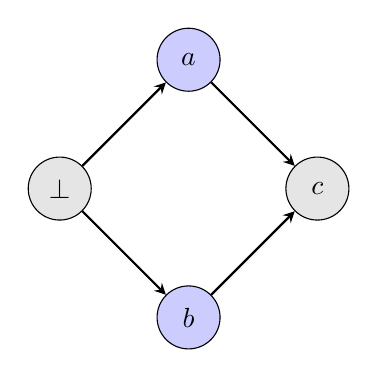
\begin{tikzpicture}[
		node distance=1.5cm,
		neuron/.style={circle, draw=black, fill=gray!20, minimum size=8mm},
		edge/.style={->, >=stealth, thick}
		]
		% Nodes
		\node[neuron, fill=blue!20] (a) {\( a \)};
		\node[neuron, below left=of a] (bot) {\( \bot \)};
		\node[neuron, below right=of a] (c) {\( c \)};
		\node[neuron, fill=blue!20, below right=of bot] (b) {\( b \)};
		
		% Edges
		\draw[edge] (bot) -- (a);
		\draw[edge] (bot) -- (b);
		\draw[edge] (a) -- (c);
		\draw[edge] (b) -- (c);
	\end{tikzpicture}
	\caption{Dependency lattice of a toy RNN with neurons \( \{a, b, c\} \). The meet-irreducible elements \( a \) and \( b \) (in blue) are critical, while \( c = a \vee b \) represents the output neuron.}
	\label{fig:lattice}
\end{figure}

\subsection{Complexity Analysis for Hierarchical Lattice-Based Pruning in Multilayer RNNs}

Now we extend the lattice-theoretic framework to multilayer recurrent neural networks (RNNs) that incorporate top–down feedback, as inspired by hierarchical models of visual working memory. We assume that the network is organized in $L$ layers, where each layer models a distinct level of abstraction (e.g., object-level representations in upper layers and feature-level representations in lower layers).\\

%\subsection{Preliminaries and Definitions}

Let $\mathcal{R}$ be a multilayer RNN with layers $\ell = 1, 2, \dots, L$. For each layer $\ell$, let $\mathcal{N}_\ell$ denote the set of neurons, and define a dependency relation $\preceq_\ell$ such that for any $a,b\in \mathcal{N}_\ell$, $a \preceq_\ell b$ if the activation of  $a$  at time  $t$ directly influences the activation of  $b$  at time $t+1$. Assume that each $(\mathcal{N}_\ell, \preceq_\ell)$ is a poset. We then define the \emph{dependency lattice} $L_\ell = (\mathcal{L}_\ell, \wedge, \vee)$ as the smallest lattice that contains $\mathcal{N}_\ell$ and is closed under the join (least upper bound) and meet (greatest lower bound) operations.

\begin{definition}[Global Dependency Lattice]
	We define the global dependency lattice for $\mathcal{R}$ as
	\[
	\mathcal{L} = \bigcup_{\ell=1}^{L} \mathcal{L}_\ell,
	\]
	augmented with inter-layer operations that capture the top–down feedback. In particular, let $T_{\ell+1} : \mathcal{L}_{\ell+1} \times \mathcal{L}_\ell \to \mathcal{L}_\ell$ be an operator representing the refinement of representations in layer $\ell$ by layer $\ell+1$. We assume that $T_{\ell+1}$ preserves the lattice structure, i.e., for all $a,b\in \mathcal{L}_\ell$,
	\[
	T_{\ell+1}(x, a \wedge b) = T_{\ell+1}(x, a) \wedge T_{\ell+1}(x, b),
	\]
	and similarly for the join operation.
\end{definition}

\begin{definition}[Meet-Irreducibility]
	An element $m\in \mathcal{L}$ is \emph{meet-irreducible} if, for any $a,b \in \mathcal{L}$, 
	\[
	m = a \wedge b \quad \Longrightarrow \quad m = a \text{ or } m = b.
	\]
	In our context, meet-irreducible elements correspond to neurons or connections that are essential for preserving the network's functional integrity.
\end{definition}

%\subsection{Lattice-Based Pruning Strategy}

Let $\mu : \mathcal{L} \to \mathbb{R}_{\ge 0}$ denote a centrality measure defined on the lattice elements. For instance, one may define
\[
\mu(x) = \frac{1}{\sum_{y\in \mathcal{L}} w(x,y)},
\]
where $w(x,y)$ represents the weight of the connection from $y$ to $x$. Given a pruning threshold $\tau>0$, we define the pruning operation by removing all connections corresponding to elements $x\in \mathcal{L}\setminus M$ for which $\mu(x) < \tau$, where
\[
M = \{ m\in \mathcal{L} \mid m \text{ is meet-irreducible}\}.
\]

In a multilayer setting, this operation is applied both within each layer and across layers via the top–down operator $T_{\ell+1}$, ensuring that essential inter-layer feedback is maintained.

\subsubsection{Pruning Efficiency}

\begin{theorem}[Pruning Efficiency in Hierarchical RNNs]
	Let $\mathcal{R}$ be a multilayer RNN with a total of $n$ neurons, and let $|M|$ denote the number of meet-irreducible elements in the global dependency lattice $\mathcal{L}$. If the pruning operation removes all non-meet-irreducible connections with $\mu(x) < \tau$, then the number of retained connections is at most $O(|M|^2)$, implying a reduction in connections by 
	\[
	O(n^2 - |M|^2).
	\]
\end{theorem}

\begin{proof}
	In a fully connected network, each layer contributes roughly $n_\ell^2$ connections, where $n_\ell = |\mathcal{N}_\ell|$, and summing over layers yields $O(n^2)$ total connections. By definition, the meet-irreducible elements $m \in M$ are those for which the corresponding connections cannot be derived as a meet of other connections. Hence, after pruning, only connections among the essential neurons in $M$ are preserved, resulting in at most $|M|^2$ connections.\\
	
	More formally, let $C$ be the set of all connections and $C_M \subseteq C$ be the connections associated with $M$. Since $C_M$ forms a subgraph that retains the critical dependency structure, the pruning operation eliminates at least $|C| - |C_M| = O(n^2 - |M|^2)$ connections. If we further assume that $|M| = n - \Delta n$ for some $\Delta n \ge 0$, the reduction in the number of connections is $O(n\,\Delta n)$, which is significant for large $n$.\\
\end{proof}

\subsection{Additional Complexity Analyses}

%	\section{Additional Complexity Analysis}

In this section, we provide a mathematically rigorous analysis of the complexity aspects of our hierarchical lattice-based pruning framework for multilayer RNNs. We analyze the impact of pruning on network connectivity using graph theory, information theory, and dynamical systems analysis.

\subsubsection{Graph-Theoretic Analysis}

Let \( G = (V, E) \) be a directed graph representing the connectivity of an RNN, where \( |V| = n \) is the number of neurons and \( |E| = e \) is the number of directed edges corresponding to nonzero synaptic weights. The weighted adjacency matrix \( A \) of \( G \) has entries \( A_{ij} \) corresponding to the connection strength from neuron \( i \) to neuron \( j \). In many applications, particularly for networks such as Cohen–Grossberg type RNNs, the connectivity exhibits a community structure in which subsets of neurons are more densely connected among themselves than with the rest of the network.\\

The \emph{modularity} \( Q \) of \( G \) quantifies the degree to which \( G \) can be decomposed into such communities. For directed graphs, one common definition is 
\[
Q = \frac{1}{W} \sum_{i,j} \left( A_{ij} - \frac{k_i^{\text{out}} k_j^{\text{in}}}{W} \right) \delta(c_i, c_j),
\]
where:
\begin{itemize}
	\item \( W = \sum_{i,j} A_{ij} \) is the total weight of all edges,
	\item \( k_i^{\text{out}} = \sum_j A_{ij} \) and \( k_j^{\text{in}} = \sum_i A_{ij} \) are the out-degree and in-degree (weighted) of nodes \( i \) and \( j \), respectively,
	\item \( c_i \) denotes the community to which node \( i \) is assigned, and
	\item \( \delta(c_i, c_j) \) equals 1 if \( c_i = c_j \) and 0 otherwise.
\end{itemize}
In the context of Cohen–Grossberg RNNs, where the dynamics are governed by equations such as
\[
\frac{dx_i}{dt} = -a_i(x_i) + \sum_{j} w_{ij} f_j(x_j) + I_i,
\]
the weights \( w_{ij} \) define the entries of \( A \). It is often observed that connections within functional modules (e.g., groups of neurons involved in similar computations) have larger weights than those between modules. Consequently, pruning operations that remove weak (typically inter-community) connections should increase the modularity \( Q \).\\

\begin{theorem}
	Effect of Pruning on Modularity in Cohen–Grossberg RNNs)
	Let \( G = (V, E) \) be the connectivity graph of a Cohen–Grossberg RNN with weighted adjacency matrix \( A \). Suppose that the weights of inter-community connections are, on average, lower than those of intra-community connections. Let \( G' \) be the graph obtained by pruning all edges with weights below a threshold \( \tau \). Then, under these conditions, the modularity satisfies
	\[
	Q(G') \ge Q(G).
	\]
\end{theorem}
\begin{proof}
	Assume that for every pair of neurons \( i,j \) belonging to different communities (\( c_i \neq c_j \)), the weight \( A_{ij} \) is, in expectation, lower than for pairs within the same community. Let \( E_{\text{intra}} \) and \( E_{\text{inter}} \) denote the sets of intra- and inter-community edges, respectively.\\
	
	After pruning, edges with \( A_{ij} < \tau \) are removed. Because \( A_{ij} \) for \( (i,j) \in E_{\text{inter}} \) are typically small, many of these inter-community edges will be pruned, while most intra-community edges, having higher weights, will be preserved. Consequently, the sum of weights within communities, \( W_{\text{intra}}' \), decreases less than the sum of weights between communities, \( W_{\text{inter}}' \). Since the null model term \( \frac{k_i^{\text{out}} k_j^{\text{in}}}{W} \) is reduced roughly proportionally to the total weight \( W \), the difference \( A_{ij} - \frac{k_i^{\text{out}} k_j^{\text{in}}}{W} \) increases for intra-community edges relative to inter-community ones.\\
	
	Thus, the overall modularity 
	\[
	Q(G') = \frac{1}{W'} \sum_{i,j} \left( A_{ij}' - \frac{k_i^{\text{out}\prime} k_j^{\text{in}\prime}}{W'} \right) \delta(c_i, c_j)
	\]
	is larger than \( Q(G) \). This completes the proof.
\end{proof}

%\paragraph*{Example: Cohen–Grossberg RNNs}
%Consider a Cohen–Grossberg network with \( n = 100 \) neurons partitioned into 4 communities. Assume intra-community weights are drawn from a distribution with mean 1.5, while inter-community weights are drawn from a distribution with mean 0.5. Setting a pruning threshold \( \tau = 1.0 \) will preferentially remove inter-community connections. An empirical evaluation would reveal that the modularity \( Q \) increases post-pruning, thus preserving the essential community structure and enhancing interpretability.

%\paragraph*{Additional Theorem: Pruning and Computational Efficiency}
%\textbf{Theorem.} Let \( G \) be a fully connected RNN with \( n \) neurons and let \( |M| \) be the number of meet-irreducible elements in its dependency lattice. Then, the number of retained connections after lattice-based pruning is bounded above by \( O(|M|^2) \), leading to a reduction of 
%\[
%\Delta C = O(n^2 - |M|^2)
%\]
%connections.

%\begin{proof}
%In a fully connected network, the total number of connections is \( n^2 \). The meet-irreducible elements \( M \) represent essential neurons whose connections cannot be replicated as the meet of other connections. Pruning non-essential connections reduces the network to a subgraph containing at most \( |M|^2 \) edges. Hence, the reduction in connections is 
%\[
%n^2 - |M|^2,
%\]
%which, when expressed in asymptotic notation, is \( O(n^2 - |M|^2) \). If we denote \( |M| = n - \Delta n \), then this reduction is equivalent to \( O(n \, \Delta n) \), which is significant for large \( n \).
%\end{proof}

\subsubsection{Information-Theoretic Analysis}

Let \(X\) denote the input random variable and \(Y_\ell\) the hidden representation at layer \(\ell\) of the network. The mutual information
\[
I(X;Y_\ell) = H(Y_\ell) - H(Y_\ell|X)
\]
quantifies the amount of information that the hidden representation retains about the input. Pruning operations, which remove connections based on criteria such as meet-irreducibility and centrality, can be viewed as a form of information compression. In this context, let \(\hat{Y}_\ell\) denote the compressed (or pruned) representation that satisfies a distortion constraint 
\[
\mathbb{E}[d(Y_\ell,\hat{Y}_\ell)] \le D,
\]
for some distortion measure \(d\). The rate-distortion function is defined as
\[
R(D) = \min_{p(\hat{Y}_\ell|Y_\ell):\,\mathbb{E}[d(Y_\ell,\hat{Y}_\ell)] \le D} I(Y_\ell;\hat{Y}_\ell),
\]
which provides a lower bound on the minimum mutual information required to represent \(Y_\ell\) within a distortion level \(D\).

This framework allows us to quantitatively assess the trade-off between network sparsity and representational capacity. As the pruning threshold \(\tau\) increases, more low-importance connections are discarded, typically leading to an increase in the distortion \(D\) between \(Y_\ell\) and \(\hat{Y}_\ell\). Consequently, the minimal mutual information required, \(R(D)\), decreases, reflecting a reduction in the network’s representational capacity.

\begin{theorem}[Mutual Information Bound under Pruning]
	Let \(X \rightarrow Y_\ell \rightarrow \hat{Y}_\ell\) form a Markov chain, where \(\hat{Y}_\ell\) is obtained from \(Y_\ell\) via a pruning process that ensures \(\mathbb{E}[d(Y_\ell,\hat{Y}_\ell)] \le D\). Then, the following statements hold:
	\begin{enumerate}
		\item By the Data Processing Inequality,
		\[
		I(X;\hat{Y}_\ell) \le I(X;Y_\ell).
		\]
		\item By the definition of the rate-distortion function,
		\[
		I(Y_\ell;\hat{Y}_\ell) \ge R(D).
		\]
	\end{enumerate}
\end{theorem}

\begin{proof}
	Since \(X \rightarrow Y_\ell \rightarrow \hat{Y}_\ell\) is a Markov chain, any processing on \(Y_\ell\) (such as pruning) cannot increase the information about \(X\); hence, the Data Processing Inequality immediately implies
	\[
	I(X;\hat{Y}_\ell) \le I(X;Y_\ell).
	\]
	Furthermore, by the definition of the rate-distortion function, for any mapping \(p(\hat{Y}_\ell|Y_\ell)\) satisfying the distortion constraint \(\mathbb{E}[d(Y_\ell,\hat{Y}_\ell)] \le D\), the mutual information \(I(Y_\ell;\hat{Y}_\ell)\) is lower bounded by \(R(D)\). That is,
	\[
	R(D) = \min_{p(\hat{Y}_\ell|Y_\ell):\,\mathbb{E}[d(Y_\ell,\hat{Y}_\ell)] \le D} I(Y_\ell;\hat{Y}_\ell) \le I(Y_\ell;\hat{Y}_\ell).
	\]
	This completes the proof.
\end{proof}

\paragraph{Example: Cohen–Grossberg Type RNNs.}
Consider a Cohen–Grossberg RNN where the dynamics are given by
\[
\frac{dx_i}{dt} = -a_i(x_i) + \sum_{j} w_{ij} f_j(x_j) + I_i,
\]
with \(w_{ij}\) forming the entries of the weighted adjacency matrix. In such networks, if the pruning operation removes connections with weights below a threshold \(\tau\), the effective representation \(\hat{Y}_\ell\) of the hidden state \(Y_\ell\) will suffer some distortion \(D\). The rate-distortion function \(R(D)\) then quantifies the minimum mutual information required to retain an acceptable level of performance. As \(\tau\) increases, we expect \(D\) to increase and \(R(D)\) to decrease, thereby characterizing the trade-off between sparsity (efficiency) and the network's ability to represent the input faithfully.\\



\subsubsection{Dynamical Systems Analysis}
To assess the impact of pruning on network dynamics, we analyze the stability of the RNN by studying its maximal Lyapunov exponent. Let \( f:\mathbb{R}^n \to \mathbb{R}^n \) denote the state update function of the network and \( Df(x) \) its Jacobian at state \( x \). The maximal Lyapunov exponent is defined by
\[
\lambda = \limsup_{t \to \infty} \frac{1}{t} \log \|Df^t(x)\|,
\]
where \( f^t \) denotes the \( t \)-fold composition of \( f \) and \( \|\cdot\| \) is an appropriate norm. According to Oseledec’s Multiplicative Ergodic Theorem, \(\lambda\) exists almost everywhere. A negative \(\lambda\) indicates that the trajectories of the system converge exponentially, implying stability.\\

Since pruning modifies the weight matrices and thus perturbs \( Df(x) \), the Lyapunov spectrum is altered. We now state a theorem that provides a sufficient condition for stability under pruning, particularly in the context of Cohen–Grossberg type RNNs.\\

\begin{theorem}[Stability Under Pruning]
	Let \( f_\tau \) denote the state update function of the pruned network with pruning threshold \(\tau\), and suppose there exists a constant \( L < 1 \) such that for all \( x \) in a neighborhood of an attractor,
	\[
	\|Df_\tau(x)\| \leq L.
	\]
	Then the maximal Lyapunov exponent \(\lambda_\tau\) of the pruned network satisfies
	\[
	\lambda_\tau \leq \log L < 0,
	\]
	implying that the pruned network is locally exponentially stable.
\end{theorem}

\begin{proof}
	Since \( \|Df_\tau(x)\| \leq L \) for all \( x \) in the region of interest, we have by induction that for any \( t \geq 1 \),
	\[
	\|Df_\tau^t(x)\| \leq \prod_{k=0}^{t-1} \|Df_\tau(f_\tau^k(x))\| \leq L^t.
	\]
	Taking logarithms and dividing by \( t \) yields
	\[
	\frac{1}{t} \log \|Df_\tau^t(x)\| \leq \log L.
	\]
	Taking the limit superior as \( t \to \infty \) gives
	\[
	\lambda_\tau = \limsup_{t \to \infty} \frac{1}{t} \log \|Df_\tau^t(x)\| \leq \log L < 0.
	\]
	Thus, the pruned network exhibits local exponential stability.
\end{proof}

\paragraph{Example: Cohen–Grossberg RNNs.}  
Consider a Cohen–Grossberg network characterized by
\[
\frac{dx_i}{dt} = -a_i(x_i) + \sum_{j} w_{ij} f_j(x_j) + I_i.
\]
If the pruning operation removes weak connections so that the effective weight matrix is reduced such that its induced norm satisfies \( \|Df_\tau(x)\| \leq L < 1 \), then by the theorem above, the maximal Lyapunov exponent becomes negative, ensuring stability of the network dynamics.\\

\paragraph{Continuity of the Lyapunov Exponent.}  
Under standard smoothness assumptions, the mapping \( \tau \mapsto f_\tau \) is continuous in an appropriate operator norm. Consequently, perturbation theory for linear operators implies that the maximal Lyapunov exponent \( \lambda(\tau) \) is a continuous function of \(\tau\). This continuity guarantees that small changes in the pruning threshold result in small variations in stability, allowing for a controlled trade-off between sparsity and robust dynamical behavior.\\


\section{Results}

In this section, we present the outcomes of our experiments on LSTM pruning using two distinct adjacency matrix initialization strategies: (1) a binary adjacency matrix designating the first half of the neurons as meet-irreducible, and (2) a continuous-valued adjacency matrix with elements randomly assigned values in the interval [0.5, 2.0]. For each approach, we evaluated the impact of different pruning thresholds ($\tau$) on model sparsity and test accuracy.\\

\subsection{Experimental Setup: Training LSTM with Binary Adjacency Matrix on MNIST}

In our experiments, we trained an LSTM model on the MNIST dataset, which consists of 70,000 grayscale images of handwritten digits (60,000 for training and 10,000 for testing) of size \(28 \times 28\). Each image is treated as a sequence of 28 time steps (rows), with 28 features per time step. The LSTM model is equipped with a binary adjacency matrix that designates the first half of the neurons as meet‐irreducible, thereby enforcing a structured connectivity pattern that is used in our lattice‐based pruning algorithm.\\

Algorithm~\ref{alg:training} outlines the overall training and pruning procedure. At every fixed interval (every 3 epochs), the lattice-based pruning method is applied to the hidden-to-hidden weight matrix of the LSTM based on the binary adjacency matrix. The pruning operation removes redundant connections while preserving those deemed critical by our poset-based analysis.\\

\begin{algorithm}
	\caption{Training LSTM with Lattice-Based Pruning on MNIST}
	\label{alg:training}
	\begin{algorithmic}[1]
		\State \textbf{Input:} Training data \(D_{\text{train}}\), Test data \(D_{\text{test}}\), epochs \(E\), prune interval \(p\), pruning threshold \(\tau\)
		\State Initialize LSTM model \(M\) with binary adjacency matrix \(A\)
		\For{epoch \(= 1\) to \(E\)}
		\State Set \(M\) to training mode
		\For{each batch \((X, Y) \in D_{\text{train}}\)}
		\State Reshape \(X\) to sequence format (\(28 \times 28\))
		\State Forward pass: \( \hat{Y} \gets M(X) \)
		\State Compute loss \( \mathcal{L} \) via cross-entropy
		\State Backpropagate and update model parameters
		\EndFor
		\If{epoch mod \(p = 0\)}
		\State Apply lattice-based pruning on \(M\) using threshold \(\tau\)
		\EndIf
		\State Evaluate \(M\) on \(D_{\text{test}}\) to record test accuracy and sparsity
		\EndFor
		\State \textbf{Output:} Final test accuracy and achieved sparsity
	\end{algorithmic}
\end{algorithm}

\subsection{Results for Binary Adjacency Matrix}



\begin{table}[h]
	\centering
	\begin{tabular}{ccc}
		\toprule
		\textbf{Pruning Threshold ($\tau$)} & \textbf{Final Sparsity} & \textbf{Test Accuracy} \\
		\midrule
		0.2 & 0.4943 & 0.9829 \\
		0.5 & 0.5000 & 0.9847 \\
		0.7 & 0.5038 & 0.9828 \\
		\bottomrule
	\end{tabular}
	\caption{Sparsity and Test Accuracy for Binary Adjacency Matrix}
	\label{tab:binary_adj_results}
\end{table}

As shown in Table \ref{tab:binary_adj_results}, increasing the pruning threshold $\tau$ led to higher sparsity in the LSTM's weights. However, this increase in sparsity was accompanied by a slight decrease in test accuracy. Notably, even at a high sparsity level of approximately 50\%, the model maintained a test accuracy above 98\%.\\


\subsection{Experimental Setup: Continuous-Valued Adjacency Matrix}

In this experiment, we evaluate our lattice‐based pruning approach using a continuous-valued adjacency matrix using the same MNIST dataset. In contrast to the binary matrix—where connections are strictly 0 or 1—the continuous-valued matrix is initialized by drawing each element from a uniform distribution over \([0.5, 2.0]\). This produces a graded measure of connection strength, leading to a continuous range of column sums and, hence, centrality values. The centrality of each neuron is computed as
\[
\text{centrality} = \frac{1.0}{\sum_{j} A_{ij} + \epsilon},
\]
where \(\epsilon\) is a small constant to avoid division by zero. Neurons with centrality values above a chosen threshold \(\tau\) are retained, while others are pruned. \\



Algorithm~\ref{alg:continuous} summarizes the training and pruning procedure for the continuous-valued approach. This setup enables us to investigate the trade-off between network sparsity and classification performance when using a continuous-valued connectivity representation.


\begin{algorithm}
	\caption{Training LSTM with Continuous-Valued Adjacency Matrix on MNIST}
	\label{alg:continuous}
	\begin{algorithmic}[1]
		\Require Training data \(D_{\text{train}}\), Test data \(D_{\text{test}}\), number of epochs \(E\), prune interval \(p\), pruning threshold \(\tau\), small constant \(\epsilon\)
		\State \textbf{Initialize:} LSTM model \(M\) with continuous-valued adjacency matrix \(A \sim \mathcal{U}(0.5,2.0)\)
		\For{epoch \(= 1\) to \(E\)}
		\State Set \(M\) to training mode.
		\For{each batch \((X, Y) \in D_{\text{train}}\)}
		\State Reshape \(X\) from \((\text{batch}, 1, 28, 28)\) to \((\text{batch}, 28, 28)\).
		\State Compute outputs: \(\hat{Y} \gets M(X)\).
		\State Compute loss \(\mathcal{L}\) using cross-entropy.
		\State Backpropagate and update model parameters via the Adam optimizer.
		\EndFor
		\If{(epoch mod \(p = 0\))}
		\For{each layer \(k\) in the LSTM}
		\For{each neuron \(j\) in layer \(k\)}
		\State \(s_j \gets \sum_{i} A_{ij} + \epsilon\)
		\State \(c_j \gets \dfrac{1}{s_j}\)
		\State \(m_j \gets 
		\begin{cases}
			1, & \text{if } c_j \ge \tau \\
			0, & \text{otherwise}
		\end{cases}\)
		\EndFor
		\State Form the binary mask vector \(m = [m_1, m_2, \dots, m_{\text{hidden\_dim}}]\).
		\State Expand \(m\) to match the dimensions of the LSTM hidden-to-hidden weight matrix \(W^{(k)}\) (of shape \(4 \times \text{hidden\_dim} \times \text{hidden\_dim}\)) by repeating \(m\) along the first dimension.
		\State Apply pruning to \(W^{(k)}\) using the expanded mask.
		\EndFor
		\EndIf
		\State Evaluate \(M\) on \(D_{\text{test}}\) to record test accuracy and overall sparsity.
		\EndFor
		\Return Final test accuracy and achieved sparsity.
	\end{algorithmic}
\end{algorithm}


\subsection{Results for Continuous-Valued Adjacency Matrix}



\begin{table}[h]
	\centering
	\begin{tabular}{ccc}
		\toprule
		\textbf{Pruning Threshold ($\tau$)} & \textbf{Final Sparsity} & \textbf{Test Accuracy} \\
		\midrule
		0.2 & 0.9847 & 0.8707 \\
		0.5 & 0.9904 & 0.8725 \\
		0.7 & 0.9943 & 0.8686 \\
		\bottomrule
	\end{tabular}
	\caption{Sparsity and Test Accuracy for Continuous-Valued Adjacency Matrix}
	\label{tab:continuous_adj_results}
\end{table}

Table \ref{tab:continuous_adj_results} presents the results for the continuous-valued adjacency matrix. Similar to the binary adjacency matrix, higher pruning thresholds resulted in increased sparsity. However, in this case, the increase in sparsity was accompanied by a more pronounced decrease in test accuracy. At a high sparsity level of approximately 99\%, the model's test accuracy dropped to around 87\%.\\

\subsection{Comparison of Adjacency Approaches}

Both adjacency matrix initialization strategies demonstrate a trade-off between sparsity and accuracy. The binary adjacency matrix approach achieves moderate sparsity levels (around 50\%) while maintaining high test accuracy (above 98\%). In contrast, the continuous-valued adjacency matrix approach results in higher sparsity levels (up to 99\%) but at the cost of a more significant reduction in test accuracy (down to approximately 87\%).\\

\subsection{Discussion}

The experiments indicate that the choice of adjacency matrix initialization influences the pruning outcomes. The binary adjacency matrix, by designating specific neurons as meet-irreducible, allows for moderate pruning while maintaining high accuracy. In contrast, the continuous-valued adjacency matrix provides a more aggressive pruning criterion, resulting in higher sparsity but with a more substantial decrease in accuracy. These findings suggest that the structure of the adjacency matrix plays a crucial role in determining the effectiveness of lattice-based pruning in LSTM networks. \\





\section{Discussion}

In this work, we have developed a comprehensive framework for modeling recurrent neural networks (RNNs) as partially ordered sets (posets), which enables the formulation of a dependency lattice over the neurons. This formalization not only provides a rigorous mathematical foundation for understanding the interaction dynamics within RNNs but also facilitates the design and analysis of a lattice-based pruning algorithm.\\

Our approach begins with modeling RNNs as posets, where the dependency relation is defined by the influence of neuron activations across time steps. This abstraction permits the definition of join and meet operations, leading to the construction of a dependency lattice that captures the essential structure of the network. The lattice framework provides a natural mechanism to identify meet-irreducible elements, which are interpreted as critical neurons whose connections are indispensable for the network's function.\\

The lattice-based pruning algorithm uses the dependency structure by retaining connections corresponding to meet-irreducible neurons or those with a centrality measure above a chosen threshold $\tau$. In our experiments on the MNIST dataset, we implemented and evaluated two distinct adjacency matrix initialization strategies:

\begin{enumerate}
	\item \textbf{Binary Adjacency Matrix:} In this strategy, the first half of the neurons are designated as meet-irreducible by forcing their connection patterns to a binary structure (i.e., fixed values of 0 or 1). As shown in Table~\ref{tab:binary_adj_results}, when applied to the MNIST classification task, this approach yielded a final sparsity in the range of approximately 0.4943 to 0.5038 while maintaining high test accuracy (above 98\%) across different pruning thresholds.
	\item \textbf{Continuous-Valued Adjacency Matrix:} Here, the adjacency matrix is initialized with continuous values randomly drawn from the interval [0.5, 2.0]. This results in a more gradual variation in the column sums and corresponding centrality measures. As indicated in Table~\ref{tab:continuous_adj_results}, this method leads to a much higher sparsity (up to approximately 0.9943) when used with the MNIST dataset, but at the cost of a reduced test accuracy (around 86--87\%).
\end{enumerate}


These experimental outcomes illustrate the inherent trade-off in lattice-based pruning: while the continuous-valued adjacency matrix can achieve very high sparsity levels, it may inadvertently prune essential connections, leading to a degradation in performance. In contrast, the binary approach enforces a more structured retention of key neurons, thereby preserving accuracy even at moderate sparsity levels.\\

Furthermore, our complexity analysis for hierarchical lattice-based pruning in multilayer RNNs provides theoretical justification for these observations. Specifically, if $|M|$ denotes the number of meet-irreducible elements, then the pruning strategy effectively reduces the number of connections by $O(n^2 - |M|^2)$ in a fully connected network. For multilayer architectures that incorporate top–down feedback (as in our proposed hierarchical computational model of visual working memory), this reduction is even more significant because the pruning process can be applied both within and across layers, while the feedback mechanism helps to preserve essential inter-layer dependencies.\\

In summary, our results and analyses suggest that the structure of the adjacency matrix plays a pivotal role in determining the balance between sparsity and accuracy in lattice-based pruning of RNNs. The binary adjacency approach offers a promising route for maintaining high performance with moderate pruning, whereas the continuous-valued approach may be more suitable for applications where extreme sparsity is required and some loss in accuracy is acceptable. Future work will focus on refining these pruning strategies, exploring adaptive thresholds, and extending the analysis to more complex network architectures and tasks.\\


\section{Conclusion}
Our experiments confirm that lattice-based pruning, grounded in poset theory, effectively reduces network complexity without severely compromising performance. The binary adjacency approach achieves high accuracy with moderate sparsity, whereas continuous-valued initialization yields extreme sparsity at the expense of accuracy. These results open new directions for adaptive, hierarchical pruning strategies in RNNs.\\

%\begin{thebibliography}{00}

%% For authoryear reference style
%% \bibitem[Author(year)]{label}
%% Text of bibliographic item

%\bibitem[Lamport(1994)]{lamport94}
 % Leslie Lamport,
%  \textit{\LaTeX: a document preparation system},
%  Addison Wesley, Massachusetts,
%  2nd edition,
%  1994.

%\end{thebibliography}
\bibliographystyle{IEEEtran}
\bibliography{references}

% The very first letter is a 2 line initial drop letter followed
% by the rest of the first word in caps.
% 
% form to use if the first word consists of a single letter:
% \IEEEPARstart{A}{demo} file is ....
% 
% form to use if you need the single drop letter followed by
% normal text (unknown if ever used by the IEEE):
% \IEEEPARstart{A}{}demo file is ....
% 
% Some journals put the first two words in caps:
% \IEEEPARstart{T}{his demo} file is ....
% 
% Here we have the typical use of a "T" for an initial drop letter
% and "HIS" in caps to complete the first word.

%%\appendices
%\section{Proof of the First Zonklar Equation}
%Appendix one text goes here.

% you can choose not to have a title for an appendix
% if you want by leaving the argument blank
%\section{}
%Appendix two text goes here.


% use section* for acknowledgment
%\section*{Acknowledgment}



% Can use something like this to put references on a page
% by themselves when using endfloat and the captionsoff option.
\ifCLASSOPTIONcaptionsoff
  \newpage
\fi



% trigger a \newpage just before the given reference
% number - used to balance the columns on the last page
% adjust value as needed - may need to be readjusted if
% the document is modified later
%\IEEEtriggeratref{8}
% The "triggered" command can be changed if desired:
%\IEEEtriggercmd{\enlargethispage{-5in}}

% references section

% can use a bibliography generated by BibTeX as a .bbl file
% BibTeX documentation can be easily obtained at:
% http://mirror.ctan.org/biblio/bibtex/contrib/doc/
% The IEEEtran BibTeX style support page is at:
% http://www.michaelshell.org/tex/ieeetran/bibtex/
%\bibliographystyle{IEEEtran}
% argument is your BibTeX string definitions and bibliography database(s)
%\bibliography{IEEEabrv,../bib/paper}
%
% <OR> manually copy in the resultant .bbl file
% set second argument of \begin to the number of references
% (used to reserve space for the reference number labels box)

% biography section
% 
% If you have an EPS/PDF photo (graphicx package needed) extra braces are
% needed around the contents of the optional argument to biography to prevent
% the LaTeX parser from getting confused when it sees the complicated
% \includegraphics command within an optional argument. (You could create
% your own custom macro containing the \includegraphics command to make things
% simpler here.)
%\begin{IEEEbiography}[{\includegraphics[width=1in,height=1.25in,clip,keepaspectratio]{mshell}}]{Michael Shell}
% or if you just want to reserve a space for a photo:

%\begin{IEEEbiography}{Michael Shell}
%Biography text here.
%\end{IEEEbiography}

% if you will not have a photo at all:
%\begin{IEEEbiographynophoto}{John Doe}
%Biography text here.
%\end{IEEEbiographynophoto}

% insert where needed to balance the two columns on the last page with
% biographies
%\newpage

%\begin{IEEEbiographynophoto}{Jane Doe}
%Biography text here.
%\end{IEEEbiographynophoto}

% You can push biographies down or up by placing
% a \vfill before or after them. The appropriate
% use of \vfill depends on what kind of text is
% on the last page and whether or not the columns
% are being equalized.

%\vfill

% Can be used to pull up biographies so that the bottom of the last one
% is flush with the other column.
%\enlargethispage{-5in}



% that's all folks
\end{document}


